

\section{Understandability Study (RQ1)}
\label{sec:understandability}
This study presents  programmers with regexes and asks comprehension questions. By comparing the understandability of semantically equivalent regexes that match the same language but have different syntactic representations, we aim to identify understandability code smells.
This study was  implemented on Amazon's Mechanical Turk with 180 participants. A total of 35 pairs of regex were evaluated. Each regex pattern was evaluated by 30 participants.
%The patterns used were designed to belong to various representations in Figure~\ref{fig:refactoringTree}.







\subsection{Metrics}
\label{sec:understadningmetric}
 We measure the understandability of regexes using two complementary metrics, \emph{matching} and \emph{compostition}.


\textbf{Matching:}
 Given a pattern and a set of strings, a participant determines by inspection which strings will be matched by the pattern. There are four possible responses for each string, \emph{matches}, \emph{not a match}, \emph{unsure}, or blank. An example from our study is shown in Figure~\ref{fig:exampleQuestion}.

 The percentage of correct responses, disregarding blanks and unsure responses, is the matching score.
 For example, consider regex pattern \verb!`RR*'!, tge five strings shown in Table~\ref{matchingmetric}, and the responses from four participants in the \emph{P1}, \emph{P2}, \emph{P3} and \emph{P4} columns.
 The {\em Oracle} indicates  the first three strings match and the last two do not. \emph{P1} answers correctly for the first three strings and the fifth, but incorrectly on the fourth, so the matching score is $4/5 = 0.80$. \emph{P2} incorrectly thinks that the second string is not a match, so the score is also $4/5 = 0.80$.  \emph{P3} marks `unsure' for the third string and so the total number of attempted matching questions is 4. \emph{P3} is incorrect about the second and fourth string, so they score $2/4 = 0.50$.  For \emph{P4}, we only have data for the first and second strings, since the other three are blank.  \emph{P4} marks `unsure' for the second string so only one matching question has been attempted;  the matching score is $1/1 = 1.00$.

Blanks were incorporated into the metric because questions were occasionally left blank in the study. Unsure responses were provided as an option so not to bias the  results through blind guessing. These situations did not occur very frequently.
%Only 1.1\% of the responses were left blank and only 3.8\% of the responses were marked as unsure.  %We refer to a response with all blank or unsure responses as an `NA'.
Out of 1800 questions (180 participants * 10 questions each), only 1.8\%(32) were impacted by a blank or unsure response (never more than four out of 30 responses per pattern).


\begin{figure}[tb]
\centering
%\includegraphics[width=0.75\columnwidth]{illustrations/ExampleQuestion}
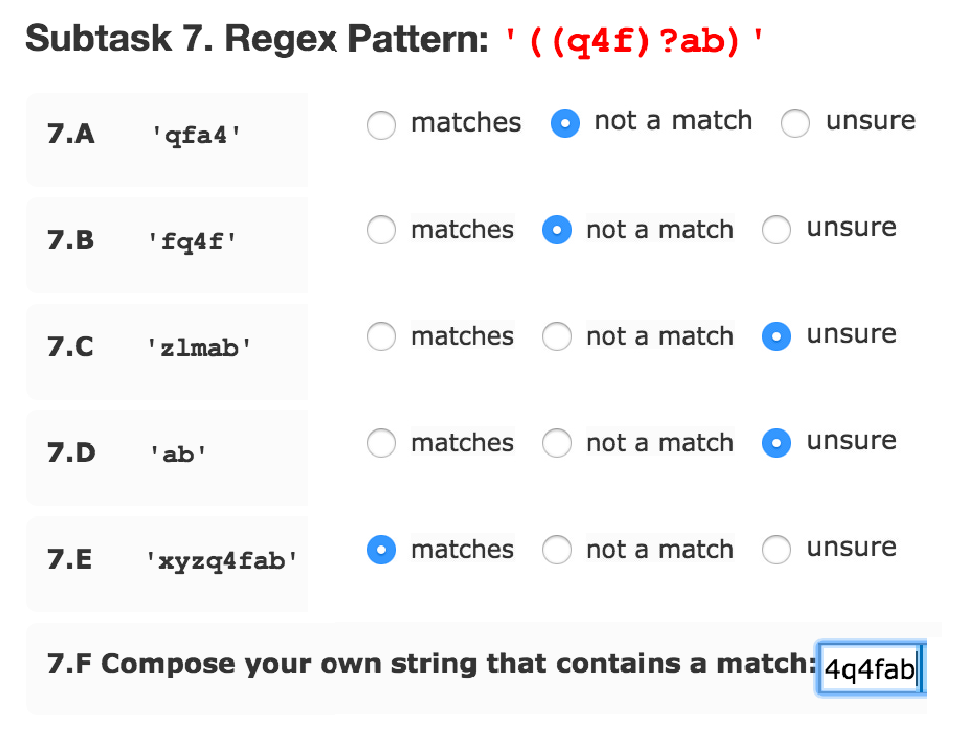
\includegraphics[width=0.75\columnwidth]{illustrations/exampleQuestion.eps}
\vspace{-12pt}
\caption{Questions from one pattern in one HIT}
\vspace{-6pt}
\label{fig:exampleQuestion}
\end{figure}



\begin{table} [t]
\caption{Matching metric example \label{matchingmetric}}
\begin{center}
%\begin{small}
\begin{tabular} {|cl | c c c c c|} \hline
\textbf{String} & \verb!`RR*'! & \textbf{Oracle} & \textbf{P1} & \textbf{P2} & \textbf{P3}& \textbf{P4}\\ \hline
1 & ``ARROW"    & \checkmark    & \checkmark    & \checkmark    & \checkmark    & \checkmark \\
2 & ``qRs"      & \checkmark    & \checkmark    & \xmark        & \xmark        & ?\\
3 & ``R0R"      & \checkmark    & \checkmark    & \checkmark    & ?             & -\\
4 & ``qrs"      & \xmark        & \checkmark    & \xmark        & \checkmark    & -\\
5 & ``98"       & \xmark        & \xmark        & \xmark        & \xmark        & -\\
\hline
  & Score       & 1.00          & 0.80          & 0.80          & 0.50          & 1.00\\ \hline
%\multicolumn{7}{l}{}\\
\multicolumn{7}{l}{\checkmark = match, \xmark = not a match, ? = unsure, -- = left blank}\\
\end{tabular}
%\end{small}
\end{center}
\vspace{-6pt}
\vspace{-6pt}
\end{table}



\textbf{Composition:}
Given a pattern, a participant composes a string they think it matches (question 7.F in Figure~\ref{fig:exampleQuestion}). If the participant is accurate, a composition score is 1, otherwise 0.  For example, given the pattern \verb!(q4fab|ab)! from our study, the string, ``xyzq4fab" matches  and gets a score of 1, but the string, ``acb" does not match and gets  a score of 0.

To determine a match, each pattern was compiled using the \emph{java.util.regex} library. A \emph{java.util.regex.Matcher} \verb!m! object was created for each composed string using the compiled pattern.  If \verb!m.find()! returned true, then that composed string was a match and scored 1, otherwise it scored 0.


\begin{table*}\begin{small}\begin{center}\caption{Averaged Info About Edges}\label{table:testedEdgesTable}\begin{tabular}
{llccccccc}
index & edge & nExp & acc1 & acc2 & cmp1 & cmp2 & Pacc & Pcmp \\
\toprule[0.16em]
E1 & C1 -- C2 & 2 & 0.94 & 0.90 & 28.0 & 27.0 & 0.268800 & 0.802400\\
E2 & C1 -- C2, T2  -- T1 & 2 & 0.84 & 0.86 & 19.5 & 27.5 & 0.751200 & 0.031185\\
E3 & C1 -- C2,T4->T1 & 2 & 0.81 & 0.86 & 15.5 & 27.5 & 0.609700 & 0.022661\\
E4 & C1->C4 & 5 & 0.76 & 0.76 & 24.2 & 23.8 & 0.555860 & 0.500942\\
E5 & C1->C5 & 5 & 0.90 & 0.88 & 27.0 & 27.2 & 0.472560 & 0.551300\\
E6 & C2->C4 & 1 & 0.83 & 0.92 & 18.0 & 20.0 & 0.075020 & 0.788800\\
E7 & C2->C5 & 4 & 0.85 & 0.86 & 26.5 & 28.5 & 0.282075 & 0.598075\\
E8 & C2->C5,T4->T1 & 2 & 0.60 & 0.82 & 11.0 & 29.0 & 0.048688 & 0.000015\\
E9 & D1->D2 & 2 & 0.84 & 0.78 & 28.0 & 26.5 & 0.306450 & 0.598350\\
E10 & D1->D3 & 2 & 0.84 & 0.87 & 28.0 & 29.0 & 0.526250 & 0.802400\\
E11 & D2->D3 & 2 & 0.78 & 0.87 & 26.5 & 29.0 & 0.155290 & 0.598350\\
E12 & L2->L3 & 3 & 0.86 & 0.91 & 27.3 & 29.3 & 0.230233 & 0.751533\\
E13 & S1->S2 & 3 & 0.86 & 0.85 & 27.0 & 26.3 & 0.420767 & 1.000000\\
E14 & T1->T3 & 3 & 0.88 & 0.86 & 21.7 & 22.7 & 0.177233 & 0.697267\\
E15 & T1->T4 & 2 & 0.80 & 0.60 & 26.0 & 11.0 & 0.049250 & 0.002759\\
E16 & T2->T4 & 2 & 0.84 & 0.81 & 19.5 & 15.5 & 0.519000 & 0.535040\\
\bottomrule[0.13em]\end{tabular}\end{center}\end{small}\end{table*}



\subsection{Design}
%\todoNow{needs to be updated with respect to no C1,T1 nodes}
We implemented this study on  Amazon's Mechanical Turk (MTurk),  a crowdsourcing platform where requesters create human intelligence tasks (HITs) for completion by workers.
%Each HIT is designed to be completed in a fixed amount of time and workers are compensated with money if their work is satisfactory. Requesters can screen workers by requiring each to complete a qualification test prior to completing any HITs.

\subsubsection{Worker Qualification}
Workers qualified to participate  by answering questions regarding some basics of regex knowledge. These questions were multiple-choice and asked the worker to analyze the following patterns: \verb!a+!, \verb!(r|z)!, \verb!\d!, \verb!q*!, and \verb![p-s]!. To pass the qualification test, workers had to answer four of the five questions correctly.

\subsubsection{Tasks}
Using the patterns in the corpus as a guide, we created 60 regex patterns that were grouped into 26 semantic equivalence groups.
 There were 18 groups with two regexes that target various edges in the equivalence classes.
The other eight semantic groups had three regexes each, forming 42 total pairs.
These semantic groups were intended to explore edges in the equivalence classes. In this way, we can draw conclusions by comparing between representations since the regexes evaluated were semantically equivalent.

To form the semantic groups, we took a regex from the corpus, matched it to a representation in Figure~\ref{fig:refactoringTree}, trimmed it down so it contained little more than just the feature of interest, and then created other regexes that are semantically equivalent but belong to other nodes in the equivalence class. For example, a semantic group with regexes \verb!((q4f){0,1}ab!, \verb!((q4f)?ab)!, and \verb!(q4fab|ab)! belong to D1, D2, and D3, respectively.
A  group with regexes \verb!([0-9]+)\.([0-9]+)! and  \verb!(\d+)\.(\d+)! is intended to evaluate the edge between C1 and C4.
We note that if we only used regexes from the corpus, we would have had regexes with different semantics at each node, or with additional language features, which would make the comparisons of the targeted features  difficult.




%Using the patterns in the corpus as a guide, we created six metagroups containing three pairs of patterns focusing on:
%\begin{itemize}
%\item S1 vs S2
%\item the digit default character class vs C1
%\item the word default character class vs C1
%\item negated digits and words vs C3, whitespace vs C2
%\item additional vs kleene repetition
%\item wrapping vs escaping literal characters
%\end{itemize}
%and four metagroups containing two triplets of patterns focusing on
%\begin{itemize}
%\item octal vs hex vs literal
%\item D1 vs D2 vs D3
%\item C1 vs C2 vs C5
%\item octal vs literal and C2 vs C5
%\end{itemize}
%
%Each of these 10 metagroups contains 6 strings, resulting in a total of 60 regex patterns.  These patterns are logically partitioned into 26 semantic equivalence groups (18 from pairs, 8 from triples).

For each of the 26 semantic groups, we created five strings for the study, where at least one matched and at least one did not match. These were used to compute the matching metric.

Once all the patterns and matching strings were collected, we created tasks for the MTurk participants as follows:
randomly select a pattern from 10 of the 26 semantic groups. Randomize the order of these 10 patterns, as well as the order of the matching strings for each pattern. After adding a question asking the participant to compose a string that each pattern matches, this creates one task on MTurk, such as the example in Figure~\ref{fig:exampleQuestion}.   This process was completed until each of the 60 regexes appeared in 30 HITs, resulting in a total of 180 total unique HITs.
%An example of a single regex pattern, the five matching strings and the space for composing a string is shown in


\subsubsection{Implementation}
Workers were paid \$3.00 for successfully completing a HIT, and were only allowed to complete  one HIT.  The average completion time for accepted HITs was 682 seconds (11 mins, 22 secs).
%A total of 241 HITs were submitted - of those 55 were rejected.
%, and 6 duplicates were ignored, always using the first accepted submission so as to obtain a value for each of the 180 distinct tasks.
A total of 54 HITs were rejected: 48 had too many blank responses, four were double-submissions by the same worker, one  did not answer the composition questions, and one was missing data for 3 questions.  Rejected HITs were returned to MTurk to be completed by others.


%
%
%
%\begin{figure}[tp]
%\begin{small}
%\fbox{\parbox{\columnwidth}{
%\begin{enumerate}
%\item
%\begin{tabular} {lrr}
%\textbf{What is your gender?} & \textbf{n} & \textbf{\%}\\ \hline
%Male & 149 & 83\%\\
%Female & 27& 15\%\\
%Prefer not to say & 4& 2\%
%\end{tabular}
%\item \textbf{What is your age?} \\
%$\mu = 31$, $\sigma = 9.3$
%
%\item
%
%\begin{tabular} {l |rr}
%\textbf{Education Level?} & \textbf{n} & \textbf{\%}\\ \hline
%High School & 5 & 3\%\\
%Some college, no degree & 46 & 26\%\\
% Associates degree & 14 & 8\%\\
%Bachelors degree & 78 & 43\%\\
%Graduate degree & 37 & 21\%\\
%\end{tabular}
%\item
%\begin{tabular} {lrr}
%\textbf{Familiarity with regexes?} & \textbf{n} & \textbf{\%}\\ \hline
%Not familiar at all & 5 & 3\%\\
%Somewhat not familiar & 16 & 9\%\\
%Not sure & 2 & 1\%\\
%Somewhat familiar & 121 & 67\%\\
%Very familiar & 36 & 20\%\\
%\end{tabular}
%\item \textbf{How many regexes do you compose each year?} \\
%$\mu = 67$, $\sigma = 173$
%\item \textbf{How many regexes (not written by you) do you read each year?} \\
%$\mu = 116$, $\sigma = 275$
%%\item In what contexts do you use regexes? \\
%\end{enumerate}
%}}
%\caption{Participant Profiles, $n=180$ \todoLast{can remove this for space} \label{participantprofile}}
%\end{small}
%\end{figure}
%


\subsubsection{Participants}

In total, there were 180 participants.
A majority were male (83\%). % with an average age of 31.
Most had
at least an Associates degree (72\%), were at least somewhat familiar with regexes (87\%), and have prior programming experience (84\%).
%On average,
%participants compose 67 regexes per year with a range from 0 to 1000.
%Participants read more regexes than they write with an average of 116 and a range from 0 to 2000.
%Figure~\ref{participantprofile} summarizes the self-reported participant characteristics from the qualification survey.


%\todoNow{in study section present choices about pairwise vs random selection for nodes.}


\subsection{Analysis}
For each of the 180 HITs, we computed a matching and composition score for each of the 10 regexes, using the metrics described in Section~\ref{sec:understadningmetric}. This allowed us to compute and then average 26-30 values for each metric  for each of the 60 regexes (fewer than 30 values were used if all the responses in a matching question were a combination of blanks and unsure). %Next, we computed average scores for matching and composition per regex.
%\todoLast{Mentioning NAs here?}


%Each regex was a member of one of 26 groupings of equivalent regexes.
%These groupings allow pairwise comparisons of the metrics values to determine which representation of the regex was most understandable and the direction of a refactoring for understandability.
Of the original 42 pairs, we report scores for only 35 pairs. Due to design flaws, seven pairs were dropped. In one, the regexes evaluated, \verb!\..*! and \verb!\.+!. are not semantically equivalent (the former is missing an escape and should be \verb!\.\.*!). In  six, the  transformations were from multiple equivalence classes and confounded. For example,  \verb!([\072\073])! is in C2 and T4 and  \verb!(:|;)! in C5 and T1;  it was not clear if any differences were due to the CCC or LIT groups, or both. However, \verb!([:;])!, could be compared with each, since it is a member of T1 and C2, so comparing it to \verb!([\072\073])! evaluates T1 and T4, and comparing to \verb!(:|;)! evaluates  C2 and C5. In the end, we covered  14 edges from Figure~\ref{fig:refactoringTree}.

To compute DFA size, we \todo{add details on how we built the DFAs for each regex}.
We use the original set of 60 regexes for the size analysis. \todo{justify this either intuitively or using the ANOVA}

\subsection{Results}
\textcolor{red}{Todo: update Table and its description, add annova and correlation analysis about representation, dfa size, and string length}

\textcolor{red}{Missing: Heatmap about the positive and negative correlation of dfa size or string length with accuracy }

Table~\ref{table:testedEdgesTable} presents the results.
\emph{Index}  enumerates the edges  evaluated in this experiment (per Figure~\ref{fig:refactoringTree}), \emph{Nodes} lists the representations, \emph{Pairs} shows the number of comparisons, \emph{Example Preferred Regex} shows a regex from the preferred node (bolded in \emph{Pairs} column), \emph{Match1} and \emph{Match2} give the matching scores for the first and second representations, respectively, and $H_0: \mu_{match1} = \mu_{match2}$ uses the Mann-Whitney test of means to compare the matching scores, and presents the p-values. The last three columns list the average composition scores for the representations and the composition p-value.

For example, consider row E5 in Table~\ref{table:testedEdgesTable}.
One pair of regexes was \verb!RR*! and \verb!R+! in L2 and L3, respectively, with average matching scores of 86\%  and 92\% and average composition scores of 97\%  and 100\%, respectively.
Thus, the community found \verb!R+! from L3 more understandable.
This is not the only regex pair in E5, however, The other is \verb!zaa*! and \verb!za+!. %, and regexes pair \verb!\..*! and \verb!\.+'!.
In aggregate, considering both regex pairs, the overall matching average for the regexes belonging to L2 was 0.86 and 0.91 for L3.
The overall composition score for L2 was 0.97 and 1.00 for L3.
The community found L3 to be more understandable than L2, from the perspective of both metrics, suggesting that L2 is generally smelly, though the differences are not significant.



%60 strings
%42 comparisons
%18@2, 8@3
%
%M6R1 ? group 3, 3 comparisons
%- 1 comparisons
%- 0 strings
%
%M3R0 ? group 3, 3 comparisons
%- 1 comparisons
%- 0 strings
%
%M3R1 ? group 3, 3 comparisons
%- 2 comparisons
%- 1 string
%
%M3R0 ? group 3, 3 comparisons
%- 2 comparisons
%- 1 string
%
%58 strings
%36 comparisons


%Although we performed 42 pairwise comparisons,

%\subsection{Results}
 In E1 through E4, there is a statistically significant difference between the representations for at least one of the metrics with $\alpha = 0.10$.  These represent the strongest evidence for code smells, suggesting that T4, D2, and C2 are less understandable.


% and we can use that to further corroborate the understandability analysis.

%\begin{table*}
%\centering
%\caption{Average Unsure Responses Per Pattern By Node (fewer unsures on the left)}\label{table:unsureResults}
%\begin{tabular}{|| l || cccc || cccc || || cccc || cccc ||}
%                & \multicolumn{4}{c||}{>=Q0(0.67)}         & \multicolumn{4}{c||||}{>=Q1(1.25)}   & \multicolumn{4}{c||}{>=Q2(1.94)}    &  \multicolumn{4}{c||}{>=Q3(2.54)}  \\ \hline
%Node     & L3 & D3 & C2 & C1 & L2 & S2 & S1 & C4 & D1 & C5 & C3 & D2 & T1 & T3 & T2 & T4 \\
%% Number of Patterns - reversed & 4 & 2 & 3 & 3 & 2 & 2 & 4 & 2 & 9 & 3 & 3 & 3 & 8 & 5 & 2 & 3\\
%Unsure Responses Per Pattern & 0.7 & 1 & 1 & 1 & 1.3 & 1.7 & 1.7 & 1.9 & 2 & 2 & 2 & 2.5 & 2.7 & 2.7 & 5.5 & 8.5\\
%\end{tabular}
%\end{table*}
Recall that participants were able to select \emph{unsure} for whether a string is matched  by a pattern.
From a comprehension perspective, this indicates some level of confusion.
For each pattern, we counted the number of responses containing at least one unsure.
%We then grouped the patterns into their representation nodes and computed an average of unsures per pattern.
%A higher number may indicate difficulty in comprehending a pattern from that node.
Overall, the highest number of unsure responses came from T4 and T2, which have octal and hex representations of characters. The least number of unsure responses were in L3 and D3.
%, which are both shown to be understandable by looking at E2 and E3 in Table~\ref{table:testedEdgesTable}.
%These nodes and their average number of unsure responses are organized by quartile in Table~\ref{table:unsureResults}.
These results mirror the understandability analysis.%, echoing that L3 and D3 are less smelly.
% for the LIT group (i.e., $\overrightarrow{T4 T1}$), the DBB group (i.e.,  $\overrightarrow{D2 D3}$), and the LWB group (i.e., $\overrightarrow{L2 L3}$) because the more understandable node has the least unsures of its group.
% The findings for D3 and D2 are contradictory, however, as  and further study is needed.
%  and the number of unsures may be too small to indicate anything, except for T2 and T4.  The one pattern from T4 that had the most unsures of any pattern (i.e., 10 out of 30) was \verb!`xyz[\0133-\0140]'!, so this may have been the least understandable pattern that we tested.
